
\section{Results}

\subsection{Blockchain Limitations}

In order to inspect the limitations imposed by the blockchain system, I created a simple testing script that checks the gas fee associated with varying model sizes.
In Table \ref{tab:gasfees}, gas fee required to perform 1 global and 10 local updates (roughly 1 round) on test blockchain setup is given for several byte sizes.
Third column gives the ratio of the current gas fee to the gas fee for 1 byte.

In the test system, all accounts start with 1000000 ETH, which is roughly equivalent to 1.2 billion dollars at the time of writing.
After 50000 byte size, we cannot do even 1 round of updates on the blockchain with this amount.

\begin{table}[h]
\centering
\label{tab:gasfees}
\begin{tabular}{r|r|r} % <-- Alignments: 1st column left, 2nd middle and 3rd right, with vertical lines in between
\textbf{Byte Size} & \textbf{Gas Fee (Gwei)} & \textbf{Ratio to Base Gas Fee} \\
\hline
1     &     736795 &  1.0000 \\
10    &     737983 &  1.0016 \\
100   &     841886 &  1.1426 \\
1000  &    1629055 &  2.2110 \\
10000 &   10457631 & 14.1934 \\
20000 &   20295764 & 27.5460 \\
30000 &   30004373 & 40.7228 \\
40000 &   39810720 & 54.0323 \\
50000 & Out of gas &  - \\
\end{tabular}
\caption{Byte Size vs. Gas Fee}
\end{table}

Therefore, our model size must be below 40000 in bytes, and around 10000 if we want to be financially reasonable.
For example, a model with 100 inputs (features), 50 neurons in a single hidden layer, and 10 outputs (classes) require $100 \times 50 + 50 \times 10 = 5500$ weights and $50 + 10 = 60$ biases, resulting in 5560 floating point numbers in total.
If we use 16, 32, or 64-bit floats, model's byte size will be 11120, 22240, and 44480 respectively.

Gas fees for communicating means and standard deviations tend to be a lot less since it's just 1D data with its length equal to the number of features.


\subsection{Experiments}

I used the dataset provided in \cite{favoriteDataset}, which contains 25192 labeled samples.
The dataset has 41 features, 3 of which are categorical.
There are 2 classes: anomaly or normal.
First, the dataset is divided into training and validation datasets with 80\%/20\% ratio, leaving approximately 20000 training samples.
After that, training samples are randomly selected and distributed equally between clients.
There are 10 clients and learning rate is $0.01$ unless otherwise specified.

At first I ran the algorithm with a single hidden layer with 50 neurons and ReLU activation function.
With $C = C_{pre} = 1$, 10 global epochs, 5 local epochs, and a batch size of 32, I got 99.17\% maximum accuracy on validation set, which varies very slightly with the given random seed.

In almost all experiments I conducted, changing the precision level of the model (16-bit, 32-bit or 64-bit floats) on the blockchain did not make any meaningful difference.
Note that this only effects how the model is communicated, not the internal representation of the model, which always uses 64-bit floats.
For example, clients get the global model from the blockchain with 16-bit floats, convert these values to 64-bit floats, do gradient descent, and report their updates to the blockchain with 16-bit floats.

I observed that the hidden layers make very little impact on the final result.
By progressively simplifying the model, I finally settled with a single linear layer $Ax + B$ with 2 neurons for output.
Despite this overly simplified model, I still get 97.28\% accuracy, and the byte size of the model is 952 with 32-bit floats or 476 with 16-bit floats.

\begin{figure}[h]
    \centering
    \begin{minipage}{.5\textwidth}
        \centering
        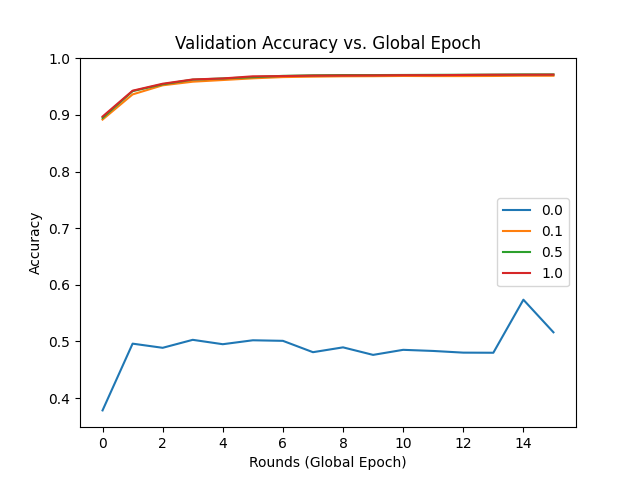
\includegraphics[width=\textwidth]{images/cpreall.png}
    \end{minipage}%
    \begin{minipage}{.5\textwidth}
        \centering
        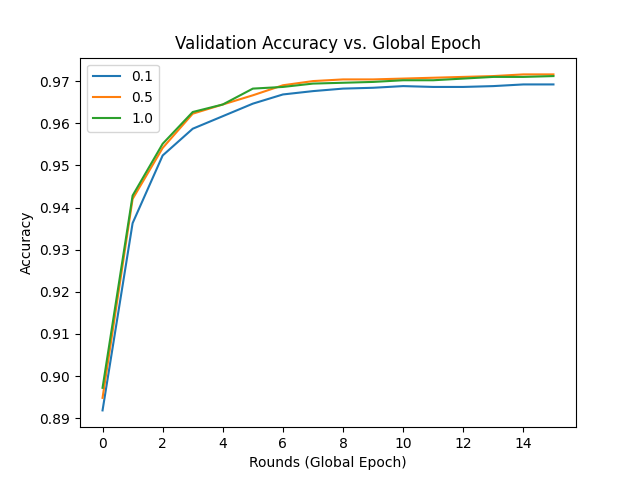
\includegraphics[width=\textwidth]{images/cpretop.png}
    \end{minipage}
    \caption{Accuracy vs. Epoch Plots with Varying $C_{pre}$}
    \label{fig:varycpre}
\end{figure}

However, data standardization proved indispensable in this dataset as accuracy plummets to ~50\% without it.
I tried different learning rates and hyperparameters but to no avail.
Furthermore, using 16-bit floats lead to NaNs without data standardization.

In Figure \ref{fig:varycpre}, I reduced the learning rate to $0.0001$, increased the global epochs to $16$, and experimented with different $C_{pre}$ parameters while keeping the rest constant.
We see that even if only one client shares $\mu_k$ and $\sigma_k$, the accuracy we attain is almost as high as the case in which all clients share standardization data.
However, I don't expect this to be the case when the data is non-IID, which is usually the case in real life.

I fixed $C_{pre}$ to $0.5$ and experimented with different $C$ values.
However, the differences were negligible.

Finally, I tested the model on 10\% of the larger KDD Cup 1999 Data \citep{kdd}, featuring 23 class labels.
Despite the increased size and complexity of the dataset, I still got ~98\% accuracy on the validation set with the single layer linear model, as long as the data standardization step is in-place.
